\section{Modular functions}

We devote the last section of this thesis to the visualization of modular functions. Without diving deeply into their theory -- which is treated  comprehensively in \Schoeneberg{} -- just enjoying the visual aesthetics of the arising figures might give an idea on the mathematical importance and beauty of modular functions.

\index{Meromorphic function}
Modular functions are meromorphic maps (\ie maps which are holomorphic\footnote{Instead of ``holomorphic'' the term ``analytic'' is also frequently used.} except for isolated poles, or in other words, maps which can be represented as quotient of two holomorphic functions) defined on the upper half-plane and satisfying a symmetry relation which is induced by the transformations of the modular group.

\begin{definition}[Modular function]
Let the upper halfplane $\mathcal{H}$ and the extended upper halfplane $\EU$ be defined as in (\ref{eqn_Upperhalfplane}) and (\ref{eqn_ExtUpperhalfplane}) respectively.
A map $f : \EU \to \EC$ is called a \emph{modular function}, if it satisfies the following conditions:
\begin{enumerate}[\quad(i)]
\item $f$ is meromorphic on the upper half-plane $\mathcal{H}$.
\item $f$ satisfies $f = f \circ A$ for all $A \in \PSL{\Z}$.
\item There exists a $k_0 \in \Z$, a sequence $(a_k)_{k \ge k_0}$, $a_k \in \C$ with $a_{k_0} \ne 0$ and a constant $C > 0$ such that $f$ has a series expansion of the form
\begin{equation*}
f(z) = \sum_{k \ge k_0} a_k \ex(k z) \quad \text{for all } z \in \C \text{ with } \Im{z} > C,
\end{equation*}
where the transformation $\ex : \C \to \C$ is defined as in (\ref{eqn_ExponentialTransform}).
\end{enumerate}
\end{definition}

\begin{figure}
\centering
\includegraphics[width=0.8\textwidth]{figures/klein-j}
\caption{The composition of the Klein modular invariant function and the inverse modified Cayley transform $j \circ \inv{\ModCayley}$.}
\label{fig_KleinJ}
\end{figure}

\begin{figure}
\centering
\begin{tabular}{c c c}

\includegraphics[width=0.45\textwidth]{figures/klein-jinv} & \quad &
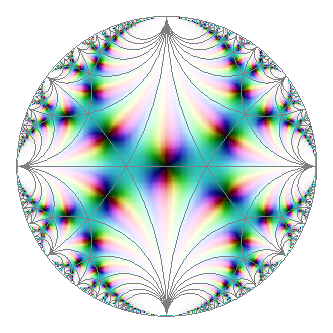
\includegraphics[width=0.45\textwidth]{figures/klein-jm1} \\
\\
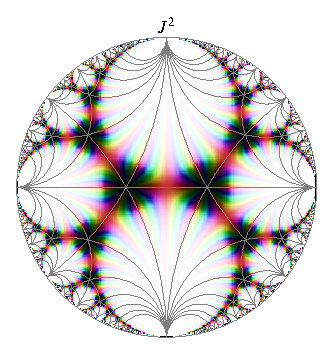
\includegraphics[width=0.45\textwidth]{figures/klein-jsqr} & \quad &
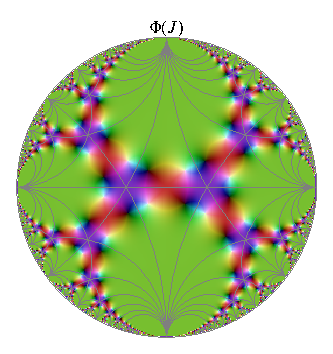
\includegraphics[width=0.45\textwidth]{figures/klein-j-mod-cayley}
\end{tabular}
\caption{The composition of the Klein modular invariant function and the inverse modified Cayley transform $j \circ \inv{\ModCayley}$.}
\label{fig_FunctionsOfJ}
\end{figure}

\begin{figure}
\centering
\includegraphics[width=0.8\textwidth]{figures/klein-jfib-large}
\caption{The composition of the Klein modular invariant function and the inverse modified Cayley transform $j \circ \inv{\ModCayley}$.}
\label{fig_KleinJFib}
\end{figure}
